% Chapter 6

\begin{savequote}[45mm]
Coconut oil for your skin \ldots
\qauthor{Polynesian proverb}
\end{savequote}

\chapter{Investigating biodiesel feedstock by SFC×GC} % Main chapter title

\label{Chapter6} % For referencing this chapter elsewhere, use \ref{Chapter6}


\section{Introduction}

Biodiesel is composed of a mixture of methyl esters of fatty acids obtained from
plant oils \autocite{SANS1935}. To comply with the relevant standard
\autocite{SANS1935}, (See chapter 3), it must consists of a mass fraction of
\SI{96.5}{\percent} or more of methyl esters, and it must have fewer than a
certain amount of specific unsaturated fatty acids methyl esters.

The methods for determining fatty acid methyl esters are chromatographic. Each
limit has its own method, and it therefore becomes expensive to determine each
of them.
 
Both these methods generate complex chromatograms that need highly skilled and
experienced chromatographers to interpret. Each peak in the chromatogram has a
retention time and area, which needs to be interpreted. There is no doubt that
the use of artificial intelligence and other technological innovation for
interpreting chromatograms will grow \todo{Cite AI chromatogram
interpretation.}, but the paradox of automation (automation helps you least when
you need it most\todo{autocite Automation paradox Strauch2018 Bainbridge1983})
predicts that as biodiesel production grows, with the implied increase in
complexity as feedstocks differentiate, the analytical chemist will need better
chemistry, in addition to better automatic data analysis.

Comprehensively coupled chromatography offers a way to better exploit chemistry
for improved separations. It does this in three ways: the first is increasing
the peak capacity of the system, the second is by improved sensitivity, and the
third is by generating patterns in the data.


\section{SFC of FAMEs}

The power of comprehensive chromatography is unlocked by orthogonality.
Orthogonality is the difference is separation mechanism in the two dimensions
\todo{autocite{LGGC nomenclature}}. When fatty acid methyl esters are separated
by a system using pure carbon dioxide as a mobile phase and unmodified silica as
a stationary phase, then the separation is according to the number of double
bonds, independent of chain length \autocite{Robertson1991, Smith1994,
Smith2001}. This is in strong contrast to the separation of FAME by GC, where
the major separation is according to volatilty, which can be adjusted, but not
overridden, by changing the polarity (or other chemical aspect) of the mobile
phase.

\begin{figure}
\centering
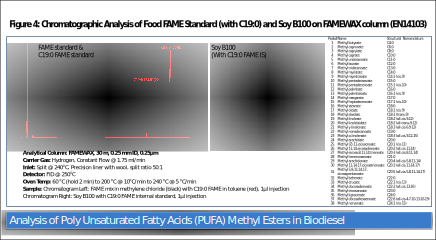
\includegraphics[width=\textwidth]{Figures/FAME-GC.pdf}
\decoRule

\caption[Separation of FAME by GC]{This figure shows that when separating FAME
by GC, using specialized column, separation is primarily by fatty acid chain
length, and secondarily by number of double bonds. Reproduced by permission of Restek Corporation.}

\label{fig:co2fill}
\end{figure}

Silver ions are often used in stationary phases to separate unsaturated
compounds, and this includes stationary phases for SFC \autocite{Sandra2002,
Potgieter2013}. The retention mechanism is quite complex
\autocite{Nikolova-Damyanova2019}, but it offers a powerful technique for the
elucidation of lipid structures, as reviewed as early as 1966
\autocite{Morris1966}. Nevertheless, in this chapter the use of stationary
phases modified with silver ions was neither necessary nor attempted.

The low viscosity of the carbon dioxide mobile phase allows for the use of very long
columns \autocite{Smith2001}.

As discussed in Section \ref{sec:Rancimat}, fatty acids are not stable at high
temperatures. This means that they might degrade during chromatographic
separation at high temperature, especially if the run times are long. Because
SFC operates at low temperatures, the labile compounds are less likely to degrade. 

\section[Benefits of fast GC]{Benefits of fast temperature programming GC for FAME analysis}

As discussed in Section \label{sec:ChromDet}, FAME can be separated by gas
chromatography using a relatively non-polar columns with high-temperature
programs. For this purpose column manufacturers supply special 'high
temperature' columns, which address two aspects of column lifetime: mechanical
degradation and stationary phase degradation. 

Fused silica has a high \keyword{tensile strength}, but also a low
\keyword{fracture toughness}. This means that it is strong enough to resist the
forces involved in its use as a column, but very liable to fracture if it gets
damaged. Very small flaws, less than a micron in depth, will cause fused silica
(or any other glass) to fracture under loads far under what would be expected
from it's tensile strength. Such flaws can be caused by mechanical scratches or
reaction with atmospheric water. Therefore the fused silica capillary is coated
in a layer of polyimide, which protects it from environmental damage. The
strength of the a capillary column therefore depends strongly on the integrity
of the polyimide coating. The polyimide, like all resins and polymers, degrade
faster at higher temperatures, so the longer the column spends at high
temperature, the shorter the overall mechanical lifetime of the column will be.
Temperature programs that minimize the time spent at high temperature will
therefore contribute to longer column lifetimes.

Column mechanical lifetime can also be improved by using metal capillaries.
Metals are not afflicted by brittle fracture the way fused silica is, but they
don't offer the chemical inertness of fused silica. But technologies have been
developed to deactivate metal surfaces \autocite{Smith2002}, which made metal
columns a modern possibility. Column manufacturers offer metal columns
specifically designed for biodiesel analysis.

Column manufacturers also minimize sta\-tion\-ary phase degradation by using
improved technologies like cross-linked resins, or polymers with backbones
resistant to certain degradation mechanisms \autocite{Day2003}.

\todo{Include column bleed mechanism?}

Short columns and fast temperature programs have a beneficial side effect:
reduced \keyword{column bleed}. Any resin- or polymer-based stationary phase
degrades over time, and this degradation is faster at higher temperatures
\autocite[p. 66]{Mcnair2019}. It is observed as a rise in baseline during the
high temperature part of a temperature program. Various stationary phase
technologies can be employed to reduce column bleed, but it should be obvious
that a \SI{1}{\metre} column will have \num{1/30}th \todo{fix ordinal} of the
column bleed of a \SI{30}{\metre} column. (It should be noted that the column
lifetime will not be longer, just that the increase in baseline signal from
column bleed will be lower.)

Another durability benefit of the coaxial stainless steel heater is that the
outer surface of the capillary column is protected from mechanical damage by
being encased. During development of the coaxial heater there were occasions
where the column was accidentally overheated by poorly-controlled resistive
heating. Even though the polyimide coating had been completely charred away and
the capillary was fragile, the column was intact and still provided good
separations.

Using carbon dioxide as coolant also protects the polyimide coating from
oxidative damage by purging the column environment of oxygen.

An aspect of fast temperature programming with such a temperature range as we're
using (\SIrange{-30}{400}{\celsius}) is \keyword{thermal shock}. Thermal shock
occurs when an object is subjected to a rapid change in temperature. Under such
non-equilibrium conditions different parts of the object will have different
temperatures. The material that the object is made of has a certain
\keyword{coefficient of thermal expansion}, which means that the relative sizes
of parts of the object will differ. This will cause stress between the parts,
and if the stress exceeds the strength of the material, the material might
fracture. Fused silica has a low coefficient of expansion \todo{autocite}, and
therefore low thermal shock, and the amount of material in a capillary is
relatively small, so we have never seen a column fail due to thermal shock.

Apart from thermal shock, there is also \keyword{thermal fatigue}. ``Thermal
fatigue (TF) is the gradual deterioration and eventual cracking of a material by
alternate heating and cooling during which free thermal expansion is partially
or completely constrained'' \autocite{Rao2001}. The expansion of the portion of
the fused silica column subjected to alternate heating and cooling is not
constrained, and the part of the fused silica column that is constrained (in the
sealing ferrules) is not subjected to alternate heating and cooling (it is held
at constant temperature in the heated T-piece block) therefore we do not expect
thermal fatigue. We did not explicitly test for the occurrence of thermal
fatigue, but we have not observed column failure due to thermal expansion.

One failure of the coaxial heater could be attributed to corrosion. The joint
between the coaxial heater and the heated T-piece block is brazed, and there was
a failure of the thin-walled stainless steel tube near that joint, in the
portion heated during the brazing operation. Visual inspection seemed to
indicate thinning caused by corrosion. An acid flux was used during the brazing,
which might have contributed to the corrosion, especially in the presence of
water from condensation of atmospheric water vapour during the cooling of the
column.

\subsection{GC Retention time precision}

To estimate the retention time variance, two aliphatic compounds (dodecane and
hexadecane) were added to the mobile phase at low concentration. These compounds
are not retained on the silica at all, and are therefore present in all the GC
runs at the same concentration, and all the peaks should therefore be identical.
Variance in peak retention, -area, and -height therefore indicate the
repeatability of the fast GC system. Variability of retention time is summarize
in Table \ref{tab:RetentionTimeVariance}

\begin{table}

\caption{\label{tab:RetentionTimeVariance}A summary of retention time repeataility of alkanes
separated on the fast temperature programmed chromatograph.}


\begin{tabular}{lllll}
Compound & n & t\textsubscript{r} (s) & S.D. of t\textsubscript{r} (s)& R.S.D. of t\textsubscript{r} (\%)\\
\hline
Dodecane & 73 & 5.07 & 0.023 & 0.46\\
Hexadecane & 73 & 6.58 & 0.052 & 0.78\\
\end{tabular}

\end{table}

The peak widths were about
\SI{500}{\milli\second}, so the \SI{20}{\milli\second} standard deviation for
hexadecane means that the variation in retention time is only about
\SI{10}{\percent} of the peak width. The relative standard deviations (RSD) of
retention times were similar to those obtained in GC×GC\cite{Shellie2002}.

\section{Experimental}


\subsection{Samples}

Various samples of vegetable oil for were obtained from supermarkets. (See Table \ref{tab:OilSamples})

\begin{table}
	\caption{Oils used for FAME analysis}
	\label{tab:OilSamples}
	\centering
	\begin{tabular}{l l}
	\toprule
	\tabhead{Oil} & \tabhead{Brand}  		\\
	\midrule
	Olive oil 		& Hojiblanca	\\
	Flax seed oil 	& Lemke 		\\
	Sunflower oil	& Pick n Pay 	\\
	Coconut oil  	& Credé Organic \\
	\bottomrule\\
	\end{tabular}
\end{table}

\subsection{Sample preparation}

Fatty acids in oils might be either free or bound to glycerol. To quantitatively
convert them to FAME therefore requires that the bound FA be transesterified,
and the FFA esterified. Both transesterification and esterification can be
achieved by acid catalyst, but this reaction is quite slow. Basic catalysts can
rapidly transesterify acyl glycerols, but will not esterify FFA.

The method we used involved first treating the oil sample with sodium hydroxide
dissolved in dry methanol. The methanol acts as a solvent but also provides an
excess of methanol so that the transesterification reaction is driven to
completion. Then an excess of acid is added, which neutralizes the base and
esterifies any free fatty acids. Then an organic solvent and water are added,
which provides two phases. The nonpolar   FAME dissolves in the organic layer,
and the polar glycerol and salts dissolve in the water layer.

\subsection{Method}

This method is based on an official method \autocite{AOCS2017}, modified in two
respects. First, the acidic catalyst boron trifluoride is replace by sulphuric
acid \todo{autocite christie}, and second, heptane is used instead of heptane.

\begin{enumerate}
  
\item Transfer \num{4} drops of melted sample to a \SI{20}{\milli\litre} glass
stoppered test tube. Add a few boiling stones

\item Add \SI{2}{\milli\litre} NaOH/Methanol solution (0.5N) and boil for
\SI{11}{\min} under reflux.

\item Add \SI{2}{\milli\litre} H\textsubscript{2}SO\textsubscript{4}/Methanol
solution via condenser and boil for \SI{2}{\minute}

\item  Add \SI{2}{\milli\litre} hexane via the condenser and boil for
\SI{1}{\minute}.

\item Remove the test tube from the heat source and leave to cool.

\item Allow phases to separate.

\item Transfer the hexane layer to a vial and use for injection.

\end{enumerate}

\subsection{SFC}

The SFC separation used no modifier. \SI{0.5}{\micro\litre} of the hexane layer
was injected as described in Section \todo{Section}. The column was five bare
silica columns in series. \todo{S}. 10-second fractions of the SFC eluate were
collected and transferred to the GC inlet via a linear restrictor.


\subsection{GC}

The fast temperature program ramped the GC column temperature from
\SI{-20}{\celsius} to \SI{350}{\celsius} in \SI{10}{s}
(\SI{2200}{\celsius\per\second}), then maintaining \SI{350}{\celsius} for
\SI{2}{\second}. Then the cooling system would activate and cool the column to
\SI{-20}{\celsius} or below, ready to trap the next SFC fraction.

In this way a series of GC chromatograms of SFC fractions were recorded, which
could be assembled into a 2D chromatogram. Figure \ref{fig:2DCanola} shows
a 2D chromatogram of a sample of FAME prepared from canola oil. This 2D
chromatogram consists of 132 fast GC chromatograms collected in approximately 90
minutes.


\begin{figure}
\centering
\includegraphics[width=\textwidth]{Figures/Interpretation.png}
\decoRule

\caption[SFC×GC of canola oil]{A 2D chromatogram of FAMEs derived from
canola oil. It is clear that the oil consists mostly of unsaturated fatty
acids.}

\label{fig:2DCanola}
\end{figure}

This chromatogram is very simple to interpret. In the SFC dimension, separation
is by number of double bonds. This means that FAMEs without double bonds elute
first in this dimension, followed by FAMEs with one, two and three double bonds
respectively. There is good resolution between the peaks in the SFC dimension. 

In the GC dimension separation is by chain length. Because these FAMEs are of
natural origin, we expect their chains to have an even number of carbon atoms.
From the literature \todo{canola oleic} we know that oleic acid (C18:1) makes up
the greatest part of canola oil, and that therefore the major peak in the
chromatogram is a C18 FAME. This allows us to easily identify the peaks for C16,
C18, C20 and C22. 

By inspecting this chromatogram we can confirm that canola oil is a viable
biodiesel feedstock: The unsaturated compounds have mostly a single double bond,
which should make it oxidatively stable, and the number of unsaturated FAMEs are
low, which means that it will most likely have suitable cold-flow properties,
because unsaturated FAMEs have higher freezing points than saturated FAMEs.


\begin{figure}
\centering
\includegraphics[width=\textwidth]{Figures/Sunflower.png}
\decoRule

\caption[SFC×GC of sunflower oil]{A 2D chromatogram of FAMEs derived from
sunflower oil. It is clear that the oil consists mostly of unsaturated fatty
acids.}

\label{fig:2DSunflower}
\end{figure}


\begin{figure}
\centering
\includegraphics[width=\textwidth]{Figures/Coconut.png}
\decoRule

\caption[SFC×GC of coconut oil]{A 2D chromatogram of FAMEs derived from
coconut oil. It is clear that the oil consists mostly of saturated fatty
acids.}

\label{fig:2DCoconut}
\end{figure}


\begin{figure}
\centering
\includegraphics[width=\textwidth]{Figures/Flax44.png}
\decoRule

\caption[SFC×GC of flax seed oil]{A 2D chromatogram of FAMEs derived from
flax seed oil. It is clear that the oil consists mostly of highly unsaturated fatty
acids.}

\label{fig:2DFlax}
\end{figure}




\todos